\documentclass[c, 10pt]{beamer}

%\usepackage{tikz}
%\usetikzlibrary{backgrounds,fit, positioning,shapes}

\usepackage{graphicx}
\usepackage{booktabs}
\usepackage{mathtools}
\usepackage{xcolor}
\definecolor{mygreen}{RGB}{35,190,35}


\newcommand\Fontvi{\fontsize{8}{7.2}\selectfont}
\newcommand\Fontci{\fontsize{7}{7.2}\selectfont}

\usepackage{colortbl}
\usepackage{rotating}
%\newlength{\NOTskip} 
%\def\NOT#1{\settowidth{\NOTskip}{\ensuremath{#1}}%
%	\hspace{0.5\NOTskip}\mathclap{\not}\hspace{-0.5\NOTskip}#1}
\usepackage{url}
\def\UrlBreaks{\do\/\do-}
\usepackage{caption}
\newcommand{\source}[1]{\caption*{\tiny Adapted from: {#1}} }
\usepackage[absolute,overlay]{textpos}


\usepackage{natbib}
\bibliographystyle{apalike}

\DeclareMathOperator*{\argmax}{arg\,max}

\usecolortheme{orchid}
\mode<presentation>
{
	\usetheme{default}      % or try Darmstadt, Madrid, Warsaw, ...
	\usecolortheme{default} % or try albatross, beaver, crane, ...
	\usefonttheme{default}  % or try serif, structurebold, ...
	\setbeamertemplate{navigation symbols}{}
	\setbeamertemplate{caption}[numbered]
} 

\addtobeamertemplate{navigation symbols}{}{%
	\usebeamerfont{footline}%
	\usebeamercolor[fg]{footline}%
	\hspace{1em}%
	\insertframenumber/\inserttotalframenumber
}

%Beamer settings
\setbeamerfont{frametitle}{size=\LARGE}
\setbeamertemplate{caption}{\raggedright\insertcaption\par}

\newcommand{\backupbegin}{
	\newcounter{framenumberappendix}
	\setcounter{framenumberappendix}{\value{framenumber}}
}
\newcommand{\backupend}{
	\addtocounter{framenumberappendix}{-\value{framenumber}}
	\addtocounter{framenumber}{\value{framenumberappendix}} 
}

\newsavebox{\authbox}
\sbox{\authbox}{%
	\centering
	\begin{minipage}{0.45\linewidth}
		\centering\normalsize
		\textit{Author}: \par
		Matteo Avigni
	\end{minipage}
	\hfill
	\begin{minipage}{0.45\linewidth}
		\centering\normalsize
		\textit{Supervisors}: \par
		Daniele Marazzina \\
		Ferdinando M. Ametrano
	\end{minipage}
}


\title{Cryptoassets in Asset Allocation:}
\subtitle{a new asset class}
\author[Matteo Avigni]{%
	\usebox{\authbox}
}

\bigskip

\institute{School of Industrial and Information Engineering \\
	Master of Science in Mathematical Engineering}
\date{29$^{\text{th}}$ April 2020}
\titlegraphic{%
	\begin{picture}(0,0)
	\put(30, 230){\makebox(0,0)[rt]{
\includegraphics[width=2cm]{Images/polimi.png}}}
	\end{picture}}

\setbeamertemplate{bibliography entry title}{}
\setbeamertemplate{bibliography entry location}{}

\begin{document}
	\AtBeginSection[]{
	\begin{frame}[noframenumbering]{Outline}
		\small \tableofcontents[currentsection, hideothersubsections]
	\end{frame} 
	}

    \begin{frame}
    	\bigskip
    	
    	\bigskip
    	
    	\bigskip
    	\large
        \maketitle
    \end{frame}
	
	\begin{frame}{Objectives}
	The main goals of this work are the following:
	\bigskip
	
		\begin{enumerate}
			\item Analyze the \textbf{state of the art} about the usage of cryptoassets in asset allocation in order to reduce portfolio volatility
			\bigskip
			
			\item Study the properties of cryptoassets as financial instruments: \textbf{correlations}, \textbf{returns} and \textbf{volatility}
			\bigskip
			\item Study the \textbf{optimal allocation} for a portfolio that contains cryptoassets and mainstream assets 
		\end{enumerate}
	\end{frame}


{
	\usebackgroundtemplate{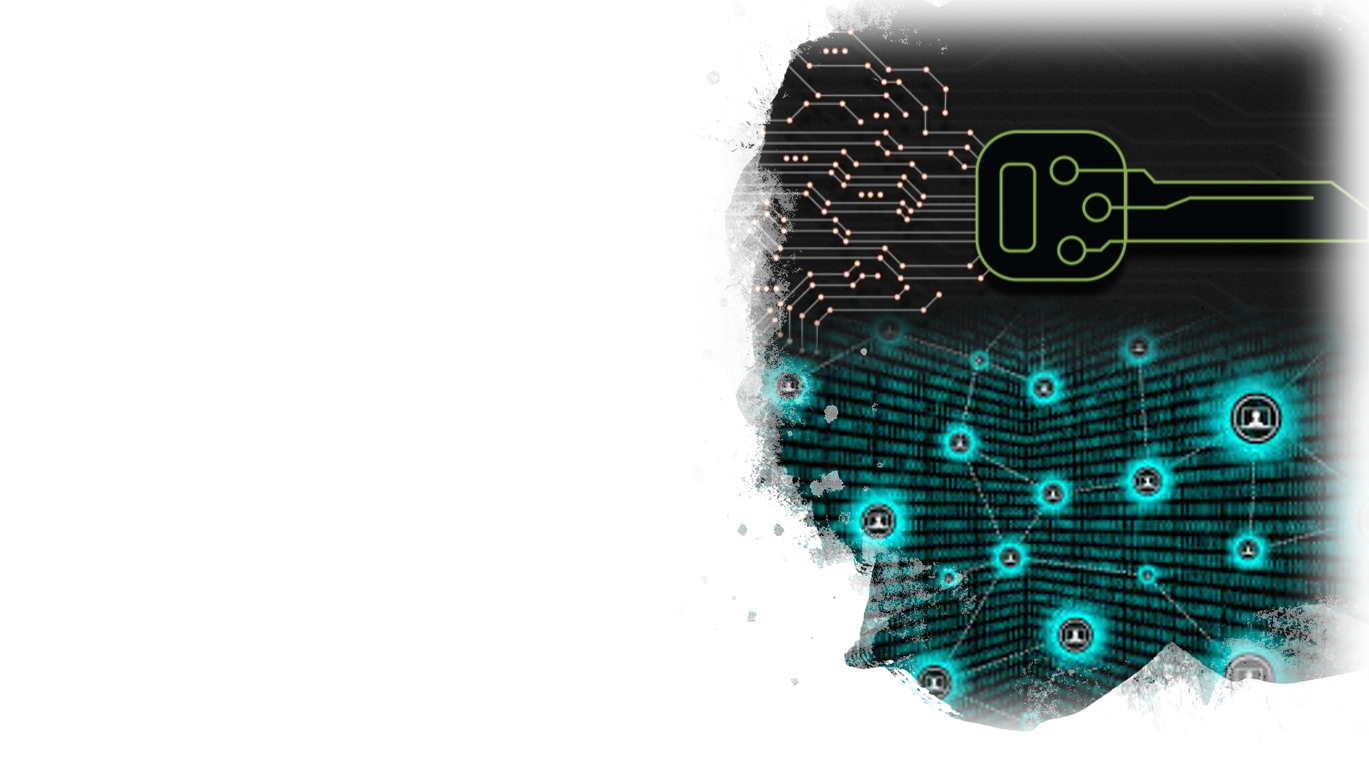
\includegraphics[width=\paperwidth]{Images/intro1}}%
	\begin{frame}{Introduction}
		 \begin{columns}[T]
			\column{.55\linewidth}			
			Cryptoassets are a type of digital assets that depend primarily on cryptography and distributed ledger technology as part of their perceived or inherent value. Since the launch of Bitcoin on the $3^{rd}$ of January 2009 a wide range of cryptoassets have been established, each one with slightly different characteristics
			\column{.45\linewidth}	
		\end{columns}
	\end{frame}
}

\begin{frame}{Introduction}
	\begin{columns}[T]
		\begin{column}{.15\linewidth}			
		\begin{figure}
			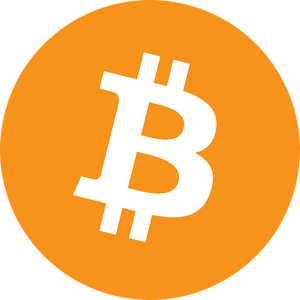
\includegraphics[height=1cm, width=1cm]{Images/btc}
		\end{figure}
		\begin{figure}
			
\includegraphics[height=1cm, width=1cm]{Images/eth}
		\end{figure}
		\begin{figure}
			
\includegraphics[height=1cm, width=1cm]{Images/ltc}
		\end{figure}
		\begin{figure}
			
\includegraphics[height=1cm, width=1cm]{Images/xrp}
		\end{figure}
		\end{column}
		\hspace{-20pt}
		\begin{column}{.35\linewidth}
		\Fontci
		\begin{tabular}{p{3.3cm}}
			\\
			The first protocol to solve the problem of \textbf{double-spending} without the need for a centralized party and to achieve \textbf{scarcity} in the digital realm \\
			\\
			\\ 
			Backed by a blockchain, the technology is aimed at a specific use case: \textbf{smart} contracts \\ 
			\\ 
			\\
			Bitcoin's closest rival in terms of the use case. There is a \textbf{limited supply} of 84 million litecoins, compared to 21 million bitcoins    \\
			\\
			A cross-border \textbf{payments solution} for large financial institutions based on blockchain technology. A transaciont of XRP can be settled in 4 seconds \\

		\end{tabular}
		\end{column}
		\vrule{}
		\hspace{10pt}
		\begin{column}{.50\linewidth}
		\begin{minipage}[c][.6\textheight][c]{\linewidth}
		More than 90\% of total volumes exchanged is covered by tha main 4 digital assets
		\begin{figure}
			\centering
			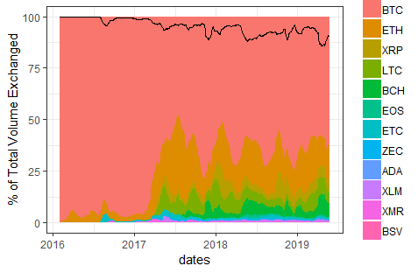
\includegraphics[height=4.4cm, width=5.5cm]{Images/volumi}
		\end{figure}
		\end{minipage}
		\end{column}	
	\end{columns}
\end{frame}



\section{Dataset}

\begin{frame}[allowframebreaks]{Dataset}
\bigskip
\Fontvi
The dataset contains 886 observations of the prices (expressed in USD) of 20 assets valued daily (excluding holidays and weekends) from the $1^{st}$ of January 2016 till the $24^{th}$ of May 2019 (some data provided by Bloomberg and others, the ones related to the cryptoassets, by Coinmarketcap).


The assets we included in our analysis are grouped into five classes:

\begin{enumerate}
	\item Cryptoassets:
	\begin{itemize}
		\Fontvi
		\item \textbf{Bitcoin} (btc): price of a single bitcoin
		\item \textbf{Ethereum} (eth): price of a single ether
		\item \textbf{Litecoin} (ltc): price of a single litecoin
		\item \textbf{Ripple} (xrp): price of a single ripple
	\end{itemize}

	\item Stock indexes:
	\begin{itemize}
		\Fontvi
		\item \textbf{S\&P500} (sp500): American stock market index based on 500 large company with stock listed either on the NYSE or NASDAQ
		\item \textbf{EUROSTOXX 50} (eurostoxx): equity index of eurozone stocks, covering 50 stocks from 11 eurozone countries
		\item \textbf{MSCI BRIC} (bric): market cap weighted index designed to measure the equity market performance across the emerging country indexes of Brazil, Russia, India and China
		\item \textbf{NASDAQ}(nasdaq): market cap weighted index including all NASDAQ tiers: Global Select, Global Market and Capital Market
	\end{itemize}
	
	\framebreak
	
	\item Bond indexes:
	\begin{itemize}
		\Fontvi
		\item \textbf{BBG Pan European} (bond\_europe): Bloomberg Barclays Pan-European Aggregate Index that tracks fixed-rate, investment-grade securities issued in different European currencies
		\item \textbf{BBG Pan US} (bond\_us): BBG US Aggregate Bond Index, a benchmark that measures investment grade, US dollar-denominated, fixed-rate taxable bond market
		\item \textbf{BBG Pan EurAgg} (bond\_eur): similar to the Pan European but it only considers securities issued in Euros
	\end{itemize} 
	\item Currencies:
	\begin{itemize}
		\Fontvi
		\item \textbf{EUR/USD} (eur): spot price of one Euro
		\item \textbf{GBP/USD} (gbp): spot price of one British Pound
		\item \textbf{CHF/USD} (chf): spot price of one Swiss Franc
		\item \textbf{JPY/USD} (jpy): spot price of one Japanese Yen
	\end{itemize}
	\item Commodities:
	\begin{itemize}
		\Fontvi
		\item \textbf{Gold} (gold): price of gold measured in USD/Oz
		\item \textbf{WTI} (wti): price of crude oil used as benchmark in oil pricing and as the underlying commodity in the NYMEX oil future contracts
		\item \textbf{Grain} (grain): S\&P GPSCI index that measures the performance of the grain commodity market
		\item \textbf{Metals} (metal): S\&P GSCI Industrial Metals index that measures the movements of industrial metal prices including aluminium, copper, zinc, nickel and lead
	\end{itemize}
\end{enumerate}
\end{frame}

\section{State of the Art}

\begin{frame}{Correlations}
	In literature there are few studies about  correlations between cryptoasstes and often the results are contradictory. They are strongly related to the time window one considers
	
	\begin{table}[H]
		\centering
		\resizebox{\textwidth}{!}{\begin{tabular}{c c}
				\begin{minipage}{.5\textwidth}
					\begin{figure}
						\centering
						\textbf{January 2013 - July 2017}\par\medskip
						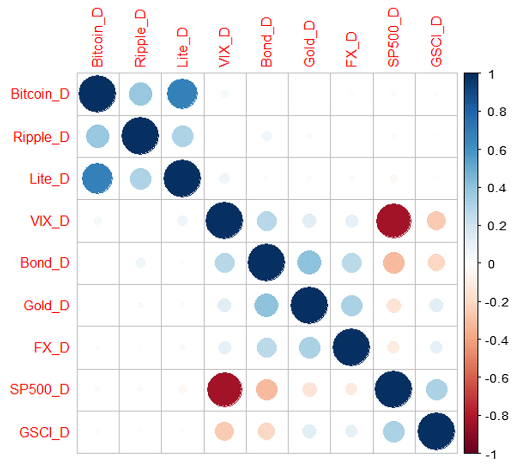
\includegraphics[height=5cm, width=5.3cm]{Images/corrcorbet}
					\end{figure}
				\end{minipage}
				&  
				\begin{minipage}{.5\textwidth}
					\begin{figure}
						\centering
						\textbf{August 2015 - April 2018}\par\medskip
						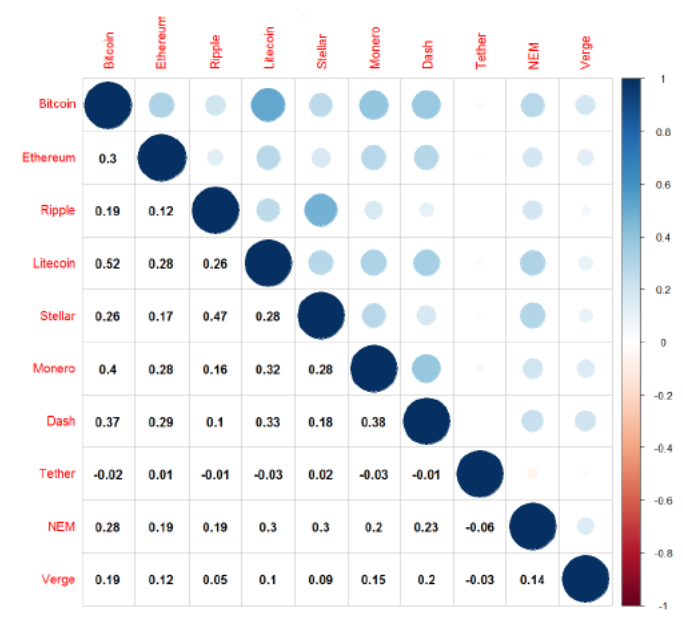
\includegraphics[height=5cm, width=5cm]{Images/corrliu}
					\end{figure}
				\end{minipage}
		\end{tabular}}
		\captionof{figure}{Correlation matrices presented in \cite{corbet} (left matrix) and \cite{weiyi} (right matrix)}
		\label{tab:liter_corr}
	\end{table}
\end{frame}



	
%\begin{frame} {More on Correlations}
%In \cite{samuele} the dataset goes from July 2010 to November 2018 and it contains %Bitcoin and several financial instruments that rapresent the asset classes. %Vengono calcolate le correlazioni di bitcoin con diversi indici di mercato usando %vari modelli per le distribuzioni dei rendimenti: 
%\bigskip
%\bigskip
%\bigskip

%	\begin{table}
%		\footnotesize
%		\centering
%		\noindent\makebox[\textwidth]{\begin{tabular}{llllllll}
%			& \begin{rotate}{45} bric \end{rotate} & \begin{rotate}{45} sp500 \end{rotate} & \begin{rotate}{45}eurostoxx \end{rotate}& \begin{rotate}{45}nasdaq \end{rotate} & \begin{rotate}{45}bond\_europe \end{rotate} & \begin{rotate}{45}bond\_us \end{rotate} & \begin{rotate}{45}bond\_eur \end{rotate}\\
%			\midrule
%			Historical Correlations & 1,4\% & 4,4\% & 4,1\% & 3,6\% & 1,4\% & -1,8\% & 1,9\% \\
%			Jump Diffusion & 2,7\% & 7,7\% & 6,3\% & 6,4\% & 1,9\% & -2,4\% & 2,7\% \\
%			Heston & 1,8\% & 6,3\% & 5,9\% & 5,4\% & 1,9\% & -2,2\% & 2,6\% \\
%			Bates & 1,5\% & 5,2\% & 4,7\% & 4,2\% & 1,4\% & -2,3\% & 2,2\% \\
%			\midrule
%		\end{tabular}
%	}

%\bigskip

%	\noindent\makebox[\textwidth]{%
%		\begin{tabular}{lllllllll}
%			& \begin{rotate}{45} eur \end{rotate} & \begin{rotate}{45} gbp \end{rotate} & \begin{rotate}{45} chf \end{rotate} & \begin{rotate}{45} jpy \end{rotate} & \begin{rotate}{45} gold \end{rotate} & \begin{rotate}{45} wti \end{rotate} & \begin{rotate}{45} grain \end{rotate} & \begin{rotate}{45} metal \end{rotate} \\
%			\midrule
%			Historical Correlations & 2,3\% & 0,7\% & 2,5\% & -1,1\% & -0,2\% & 0,8\% & 3,5\% & 2,7\% \\
%			Jump Diffusion & 2,7\% & 1,2\% & 4,4\% & -1,8\% & -0,6\% & 1,1\% & 4,2\% & 4,2\% \\
%			Heston & 2,8\% & 0,9\% & 3,2\% & -1,8\% & -0,5\% & 0,9\% & 4,5\% & 3,3\% \\
%			Bates & 3,1\% & 0,5\% & 2,5\% & -1,2\% & -0,1\% & 1,0\% & 3,3\% & 2,8\% \\
%			\midrule
%	\end{tabular}}
%	\end{table}

%A further analysis done by the author is to compute the 18-months and 36-months rolling correlation between Bitcoin and the indexes. The correlations of any asset with Bitcoin is hardly ever significantly different from zero, and when it is, its absolute level is never greater than 15\% unless for a small period.
%\end{frame}
	
\begin{frame}{Markowitz Model}
The \textbf{Efficient Frontier} is the set of portfolios which satisfy the condition that no other portfolio exists with a higher expected return but with the same standard deviation of return. One can obtain this set by solving the following quadratic problem and by taking the positively sloped portion of the resulted hyperbola:
    \begin{equation}
        \begin{aligned}
        \min_{w \in \mathcal{W}} \quad & \frac{1}{2}w^t \Sigma w\\
        \textrm{s.t.} \quad & \mathop{\mathbb{E}}\left[ R_p  \right] = \mu\\
        & e^T w = 1    \\
        \end{aligned}
    \end{equation}
for $\mu \in \left( -\inf, \inf \right)$.
\end{frame}
\begin{frame}{Efficient Frontiers}
	In \cite{samuele} the dataset goes from July 2010 to November 2018 and it contains Bitcoin and several financial instruments that rapresent the asset classes. The author computed  efficient frontier with the usual objective function and with the CVaR objective function:
	\begin{columns}
		\begin{column}{0.5\textwidth}
			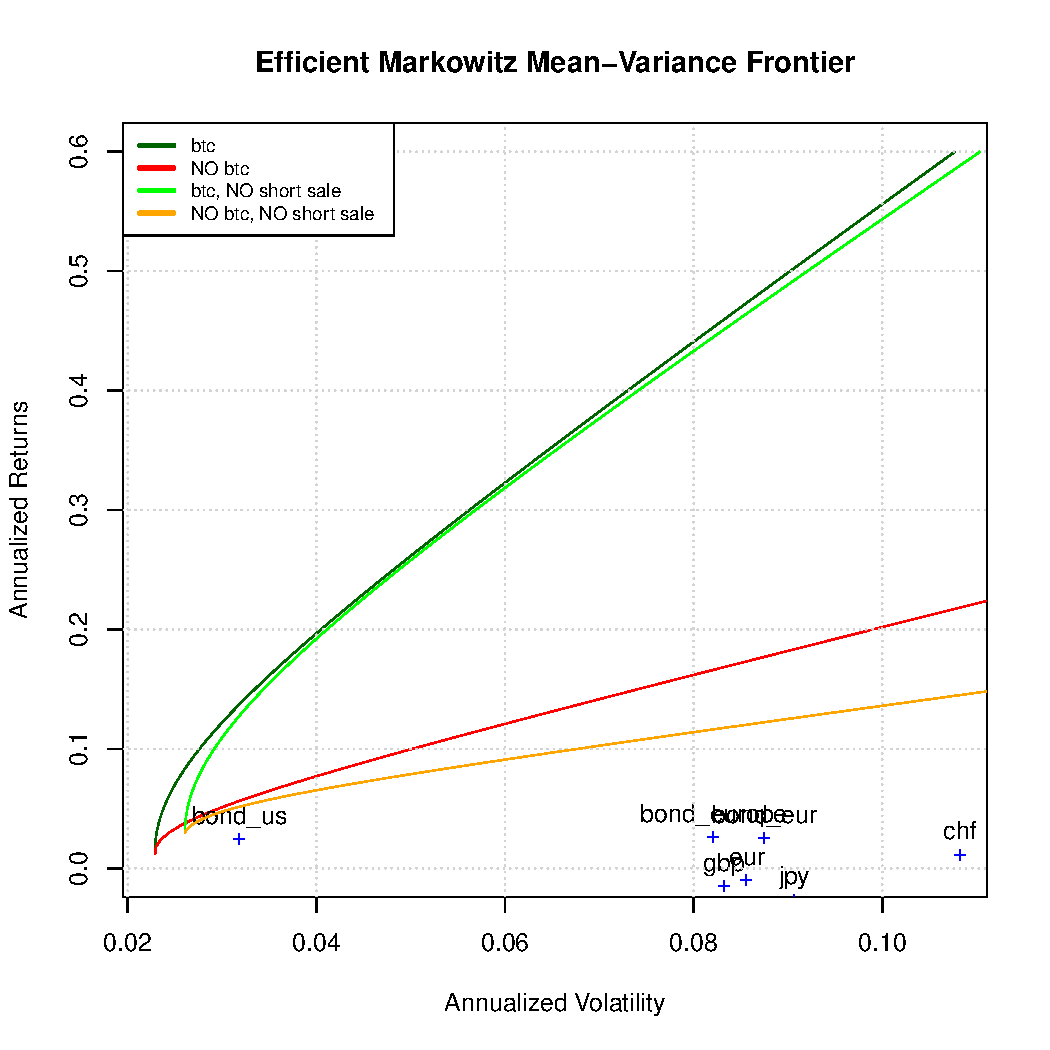
\includegraphics[width=\textwidth]{Images/efficient_frontier}
		\end{column}
		\begin{column}{0.5\textwidth}  %%<--- here
			%		\centering
			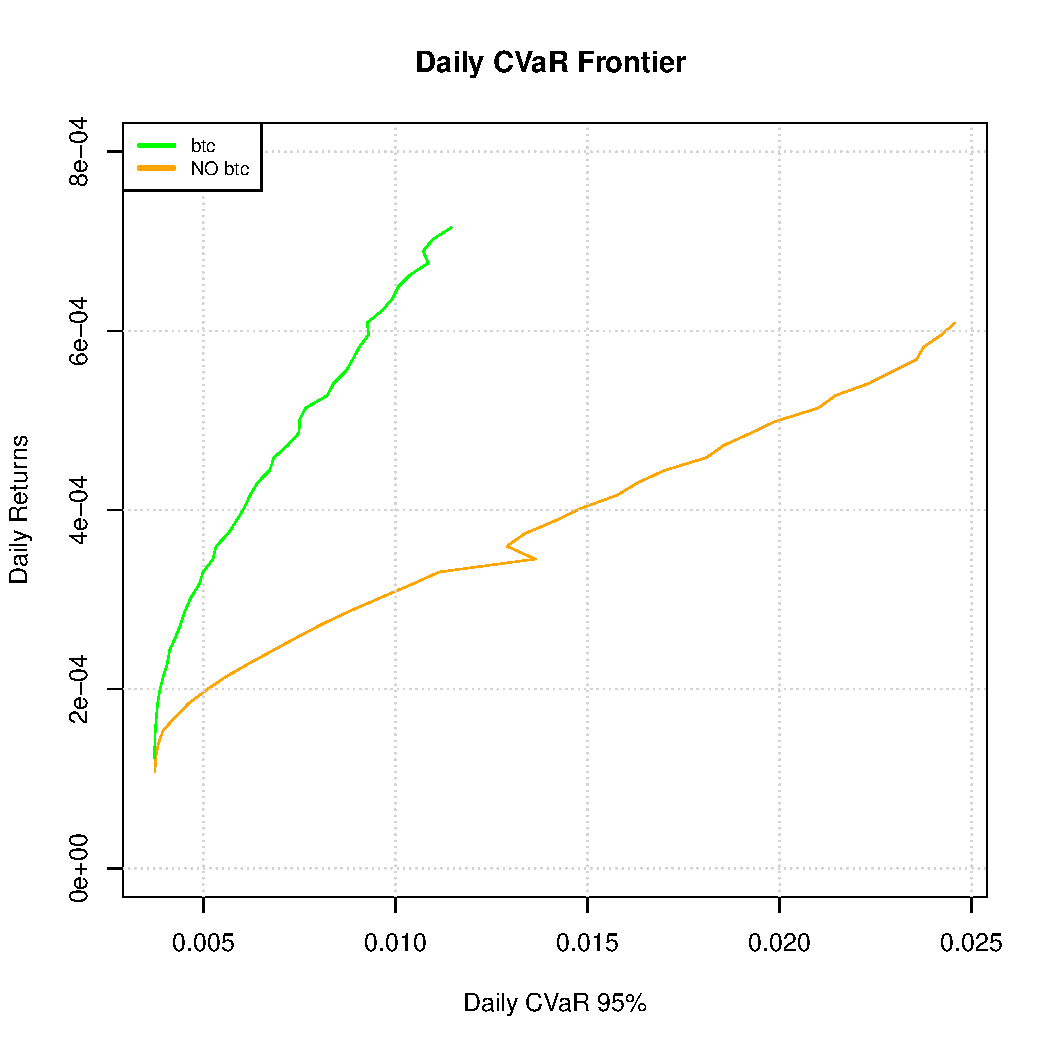
\includegraphics[width=\textwidth]{Images/efficient_frontier_CVaR}
		\end{column}
	\end{columns}
	In both cases including bitcoin is a winning strategy.
\end{frame}

\section{Cryptoassets properties}

\subsection{Correlations}
\begin{frame}{Empirical Correlations}
	The empirical correlation is computed using Pearson's sample correlation formula on the daily log-returns obtained from the price dataset.
	\begin{figure}
		\centering
		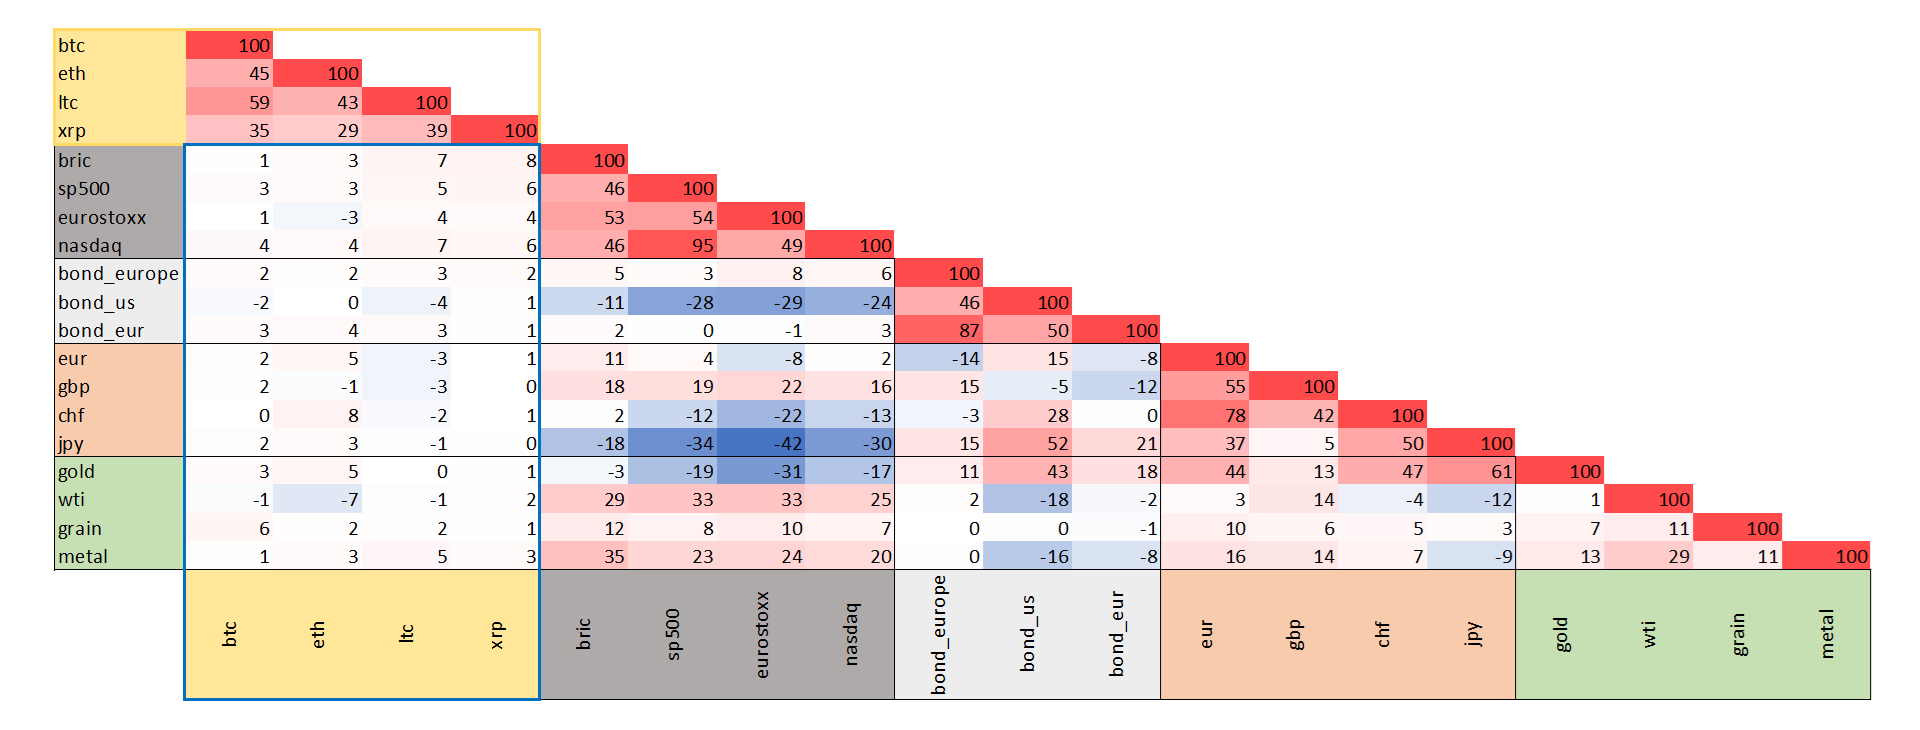
\includegraphics[width=10cm,trim=4 4 4 4,clip]{Images/empcorr}
	\end{figure}
	The results clearly show that:
	\begin{itemize}
		\item Cryptoassets has low correlation with every other asset
		\item Assets in the same class usually have a high correlation among them
	\end{itemize}
\end{frame}
\begin{frame}{P-Values}
	We then computed the significance of historical correlations through Pearson's t-test and Permutation test:
	\begin{figure}
		\centering
		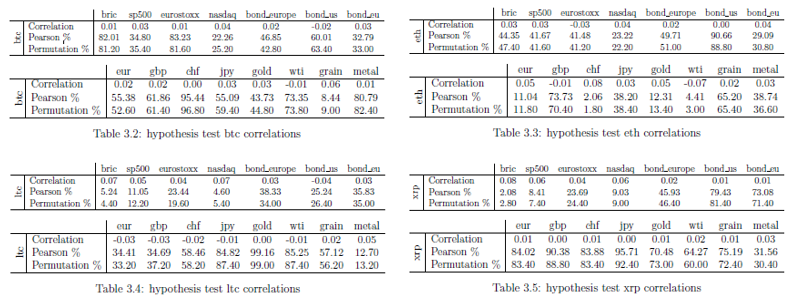
\includegraphics[width=11cm]{Images/sigtable}
	\end{figure}
	In almost every case there is no statistical evidence that correlations are different from zero and when this is the case, the correlations are always below 0.1 in absolute value
\end{frame}
\begin{frame}{Bitcoin Rolling Correlations}
Equities
\begin{figure}
	\centering
	\noindent\makebox[\textwidth]{
			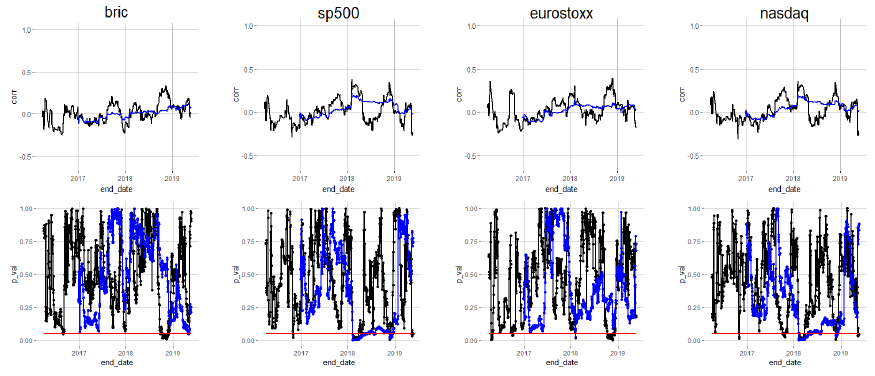
\includegraphics[width=1\linewidth]{Images/rollcorreqt}
	}
\end{figure}
\end{frame}
\begin{frame}{Bitcoin Rolling Correlations}
Bonds
\begin{figure}
	\centering
	\noindent\makebox[\textwidth]{
		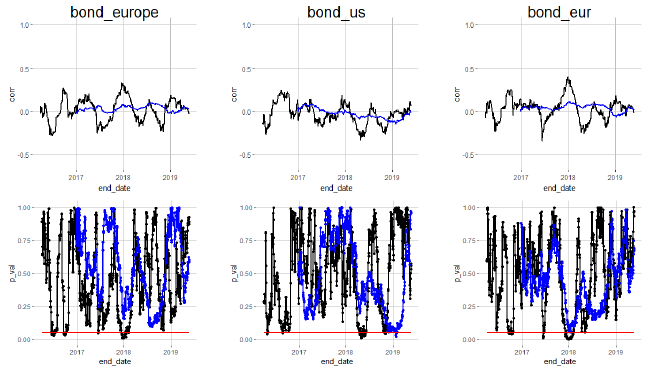
\includegraphics[width=0.9\linewidth]{Images/rollcorrbond}
	}
\end{figure}
\end{frame}
\begin{frame}{Bitcoin Rolling Correlations}
Currencies
	\begin{figure}
		\centering
		\noindent\makebox[\textwidth]{
			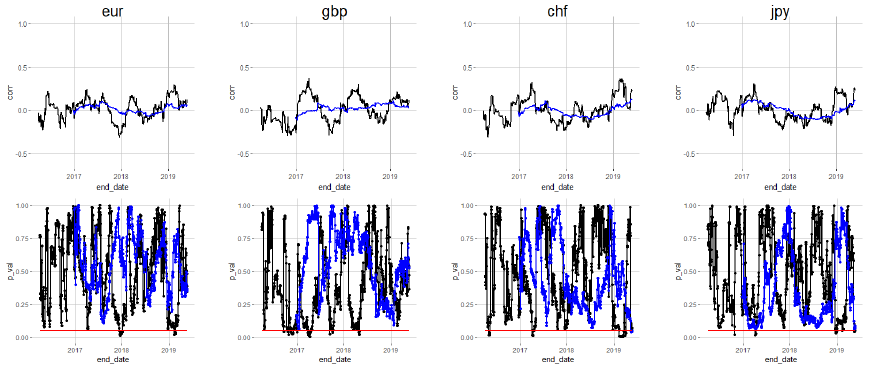
\includegraphics[width=1\linewidth]{Images/rollcorrcur}
		}
	\end{figure}
	\end{frame}
\begin{frame}{Bitcoin Rolling Correlations}
    Commodities
	\begin{figure}
		\centering
		\noindent\makebox[\textwidth]{
			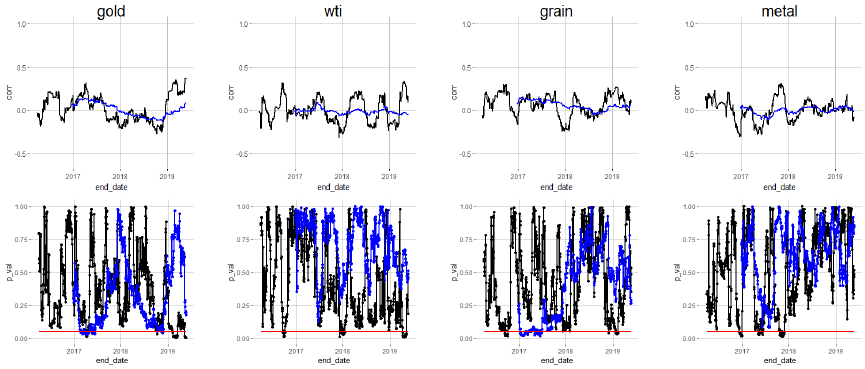
\includegraphics[width=1\linewidth]{Images/rollcorrmat}
		}
	\end{figure}
\end{frame}
\begin{frame}{Cryptoassets Rolling Correlations}
	\begin{figure}
		\centering
		\noindent\makebox[\textwidth]{
			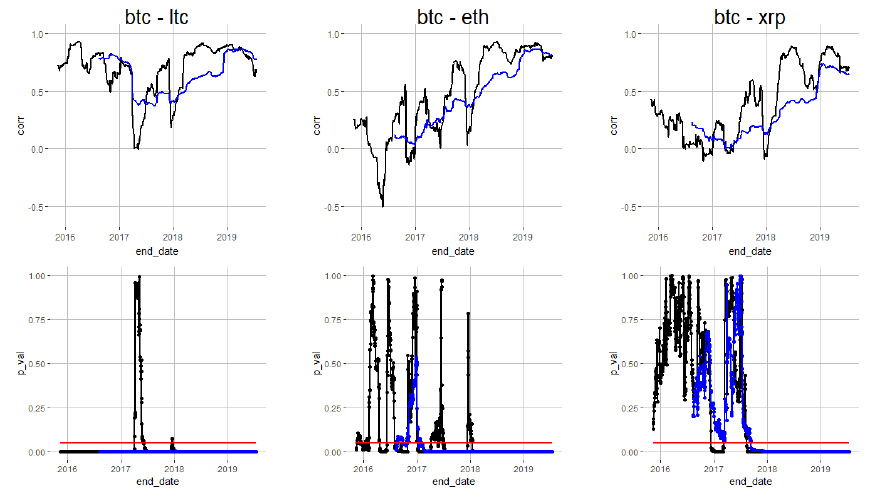
\includegraphics[width=0.9\linewidth]{Images/rollcorrcrypto1}
		}
	\end{figure}
\end{frame}
\begin{frame}{Cryptoassets Rolling Correlations}
	\begin{figure}
		\centering
		\noindent\makebox[\textwidth]{
			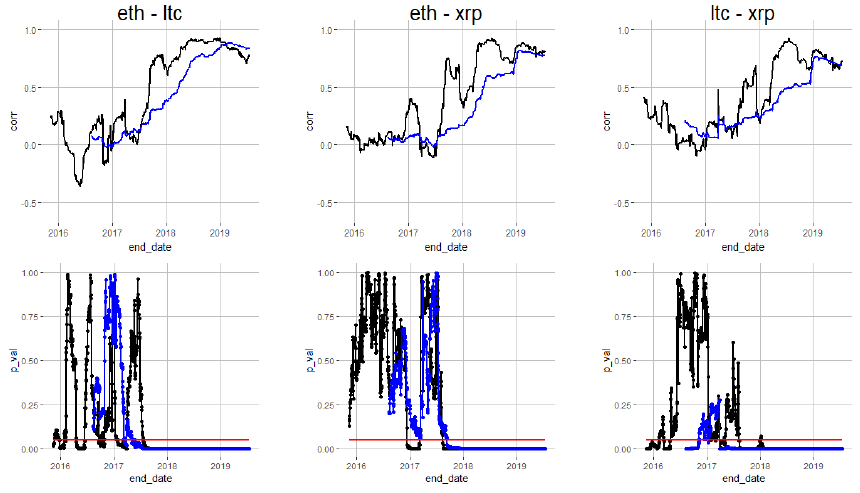
\includegraphics[width=0.9\linewidth]{Images/rollcorrcrypto2}
		}
	\end{figure}
\end{frame}

\subsection{Stylized Facts}
\begin{frame}{Returns Distribution}
Are returns of cryptoassets \textbf{i.i.d.}?
	\begin{columns}
		\begin{column}{0.5\textwidth}
		\begin{figure}
			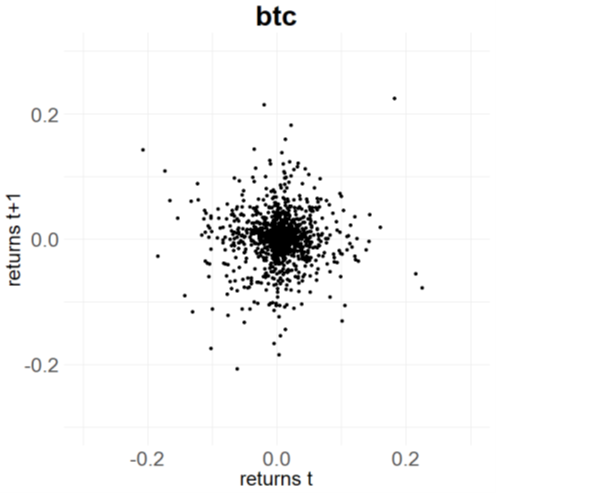
\includegraphics[width=3.4cm]{Images/lagbtc}
		\end{figure}
		\begin{figure}
			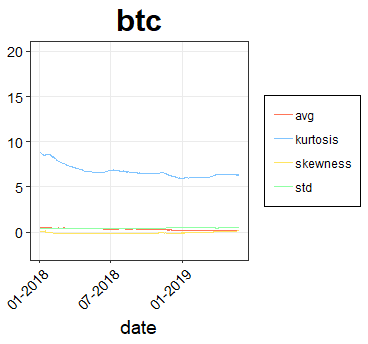
\includegraphics[width=4cm]{Images/btc _lag1d_200.png}
		\end{figure}
		\end{column}
		\begin{column}{0.5\textwidth}  %%<--- here
			%		\centering
		\begin{figure}
			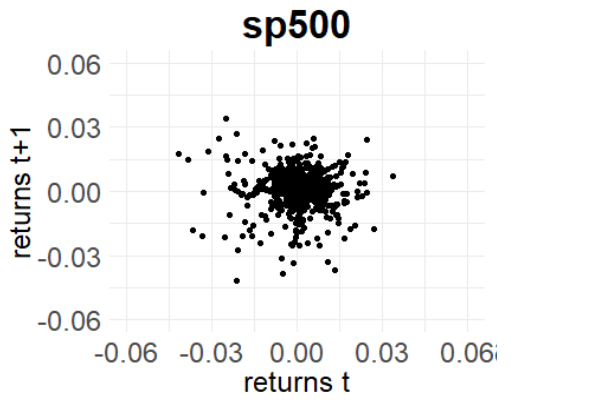
\includegraphics[width=3.6cm, height=2.8cm]{Images/lagsp500}
		\end{figure}
		\begin{figure}
			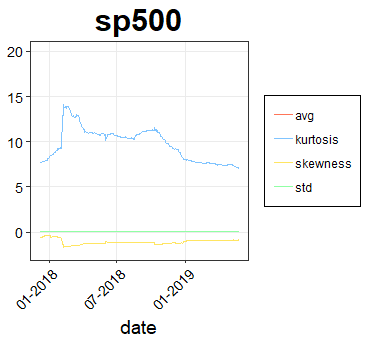
\includegraphics[width=4cm]{Images/sp500 _lag1d_200}
		\end{figure}
		\end{column}
	\end{columns}
	The distribution parameters are calculated on a 2-years rolling window
\end{frame}
\begin{frame}{Return Distribution}
But they also have the same drawbacks of standard assets' returns
	\begin{columns}
		\begin{column}{0.5\textwidth}
		\centering
		\bigskip
		
		Fat Tails
		\begin{figure}
			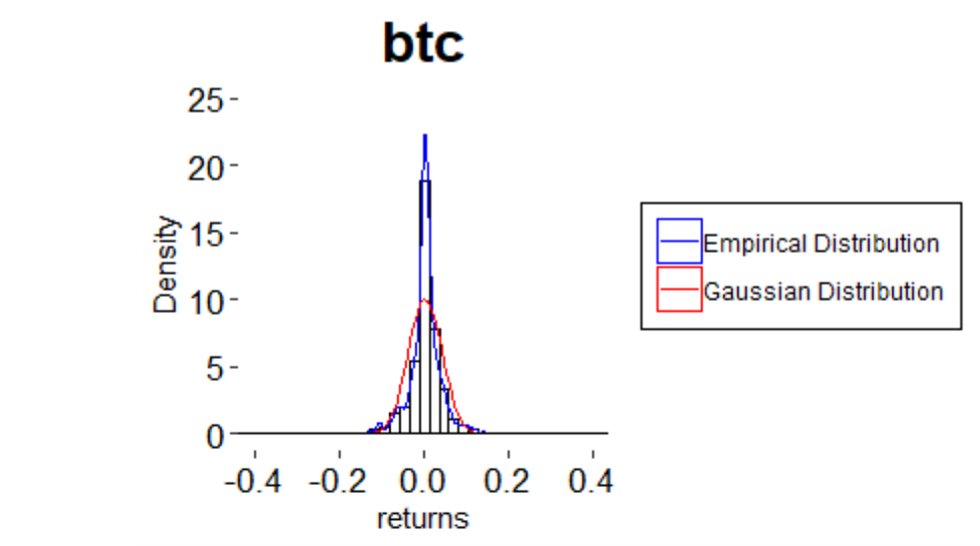
\includegraphics[width=4cm]{Images/distrbtc.png}
		\end{figure}
		\begin{figure}
			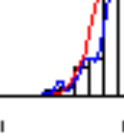
\includegraphics[width=1.3cm]{Images/codasinistra}
			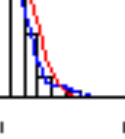
\includegraphics[width=1.3cm]{Images/codadestra}
		\end{figure}
		\end{column}
		\begin{column}{0.5\textwidth}  
		\centering
		Volatility Clustering
		\begin{figure}
			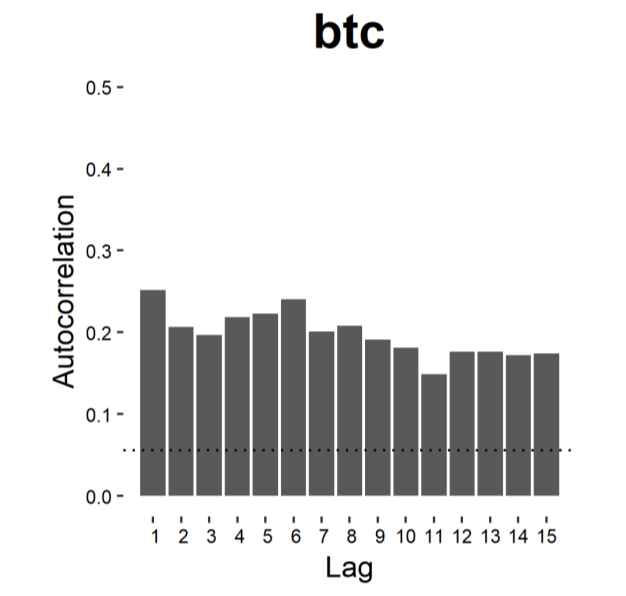
\includegraphics[width=4cm, height=3.1cm]{Images/clust}
		\end{figure}
		\end{column}
	\end{columns}
\end{frame}

\section{Optimal Allocation}
\begin{frame}{Efficient Frontiers}
	\begin{columns}
		\begin{column}{0.5\textwidth}
		    \Fontvi{} From the $1^{st}$ of January 2016 till the $24^{th}$ of May 2019
			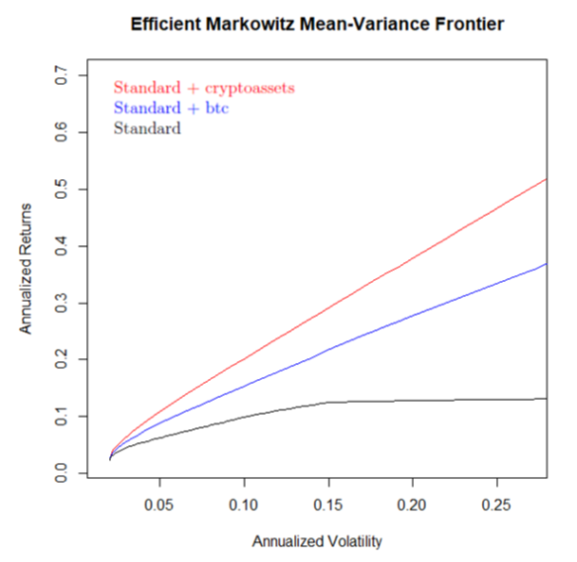
\includegraphics[width=5cm]{Images/effwhole}
		\end{column}
		\begin{column}{0.5\textwidth}
		    \Fontvi{} From the $14^{th}$ of July 2017 till the $24^{th}$ of May 2019
			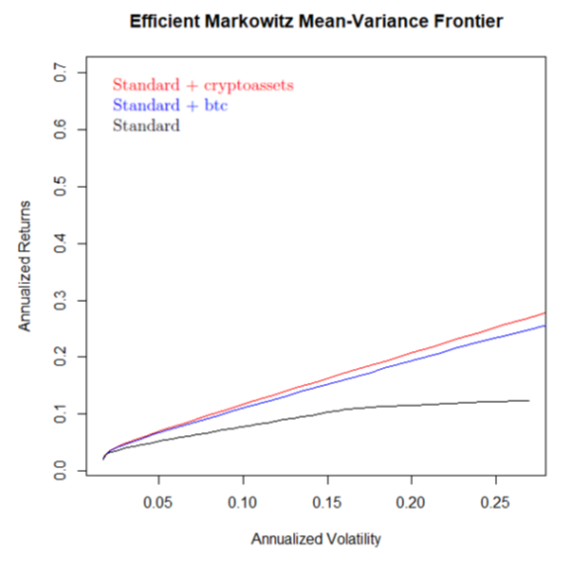
\includegraphics[width=5cm]{Images/effhalf}
		\end{column}
	\end{columns}
	\begin{center}
	    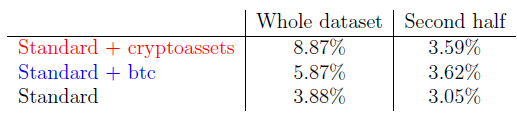
\includegraphics[width=5cm]{Images/sharpe.png}
	\end{center}
\end{frame}



%torte






%rolling allocation

\begin{frame}{Optimal Portfolio}
Best Sharpe Ratio portfolios are allocated as below:
	\begin{columns}
		\begin{column}{0.1\textwidth}
		    \bigskip
		    \bigskip
		    
            \Fontvi{}Whole data set
            \bigskip
            \bigskip
            \bigskip
            \bigskip
            \bigskip
            \bigskip
            \bigskip
            
            
            \Fontvi{}Half data set
		\end{column}
		\begin{column}{0.3\textwidth}  
		    \begin{center}
            \Fontvi{}\textcolor{red}{Standard + cryptoassets}
            \end{center}
            \begin{figure}
                \centering
                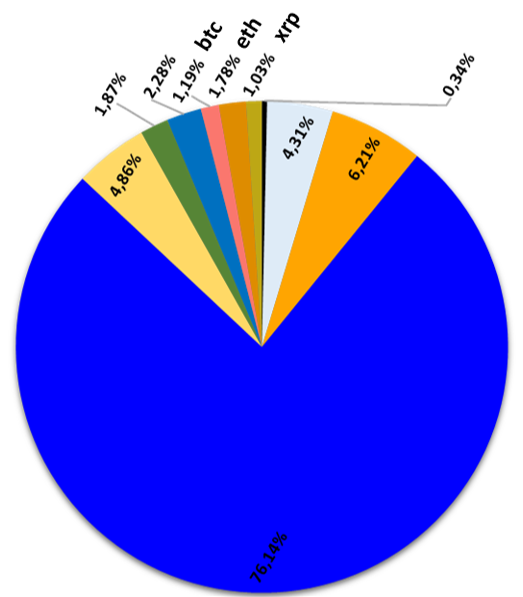
\includegraphics[width=2.55cm]{Images/torte/torta_whole_tutte.png}
            \end{figure}
            \begin{figure}
                \centering
                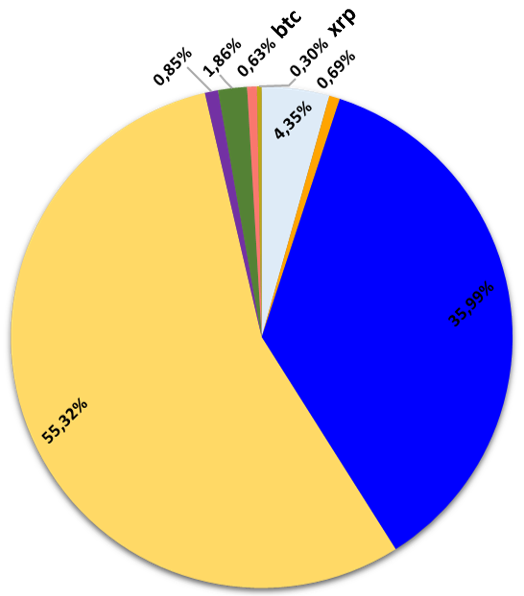
\includegraphics[width=2.55cm]{Images/torte/torta_half_tutte.png}
            \end{figure}
		\end{column}
		\begin{column}{0.3\textwidth}  
		    \begin{center}
            \Fontvi{}\textcolor{blue}{Standard + btc}
            \end{center}
            \begin{figure}
                \centering
                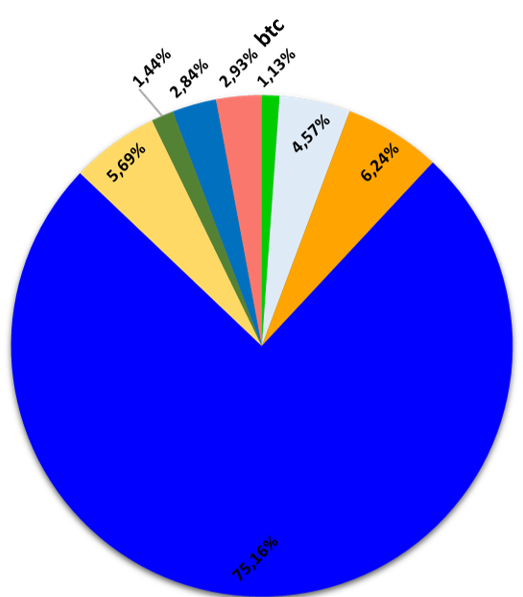
\includegraphics[width=2.55cm]{Images/torte/torta_whole_btc.png}
            \end{figure}
            \begin{figure}
                \centering
                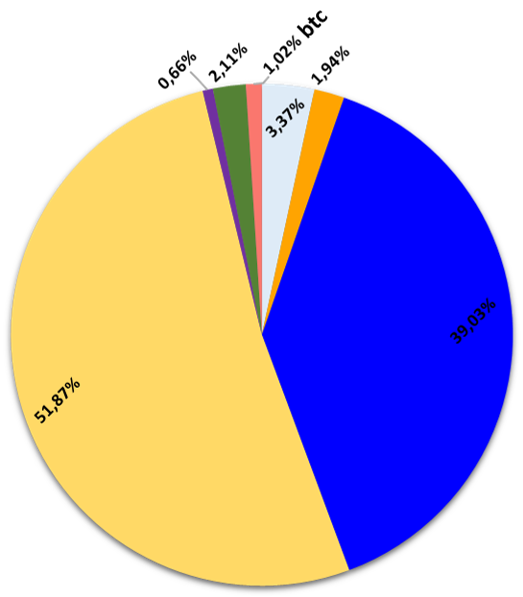
\includegraphics[width=2.55cm]{Images/torte/torta_half_btc.png}
            \end{figure}
		\end{column}
    	\begin{column}{0.3\textwidth} 
    	    \begin{center}
            \Fontvi{}Standard
            \end{center}
            \begin{figure}
                \centering
                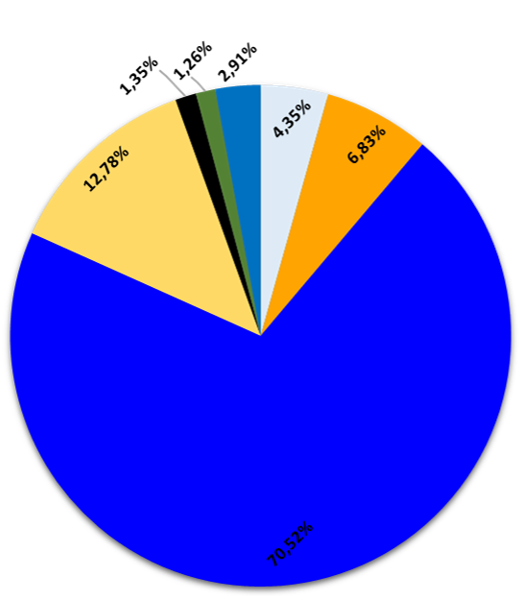
\includegraphics[width=2.55cm]{Images/torte/torta_whole_no.png}
            \end{figure}
            \begin{figure}
                \centering
                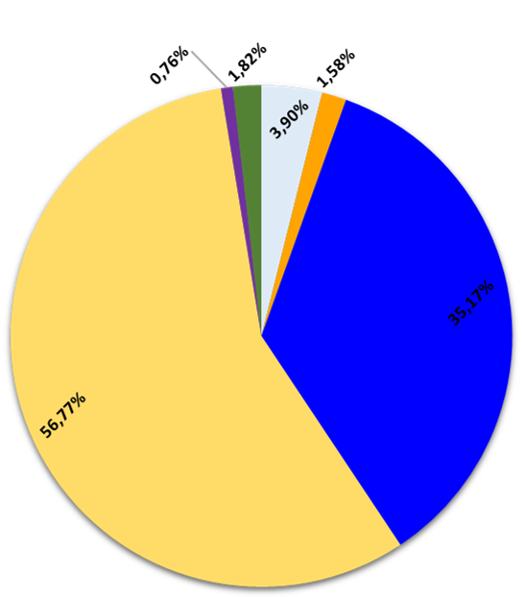
\includegraphics[width=2.55cm]{Images/torte/torta_half_no.png}
            \end{figure}
		\end{column}
	\end{columns}
	\begin{figure}
	    \centering
	    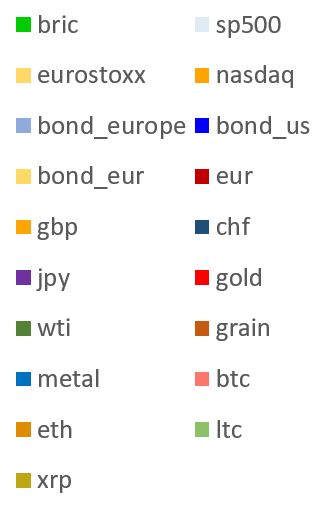
\includegraphics[width=\linewidth]{Images/legend.PNG}
	\end{figure}
\end{frame}

\begin{frame}{Rolling Optimal Portfolios}
2-years rolling time windows for the optimal portfolio, smoothed with a monthly time window:
	\begin{columns}
		\begin{column}{0.1\textwidth}
		    \bigskip
		    \bigskip
		    
            \Fontci{}Focus on cryptoasset
            \bigskip
            \bigskip
            \bigskip
            \bigskip
            \bigskip
            
            
            \Fontci{}Focus on Standard Asset
		\end{column}
		\begin{column}{0.3\textwidth}  
		    \begin{center}
            \Fontvi{}\textcolor{red}{Standard + cryptoassets}
            \end{center}
            \begin{figure}
                \centering
                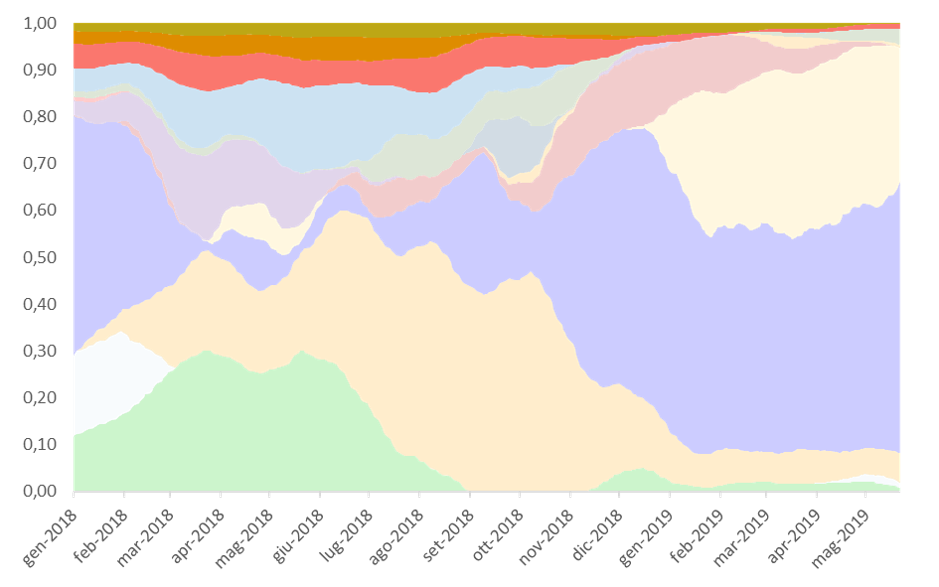
\includegraphics[width=3.2cm, height=2.6cm]{Images/rolling_allocation/rollcrall.png}
            \end{figure}
            \begin{figure}
                \centering
                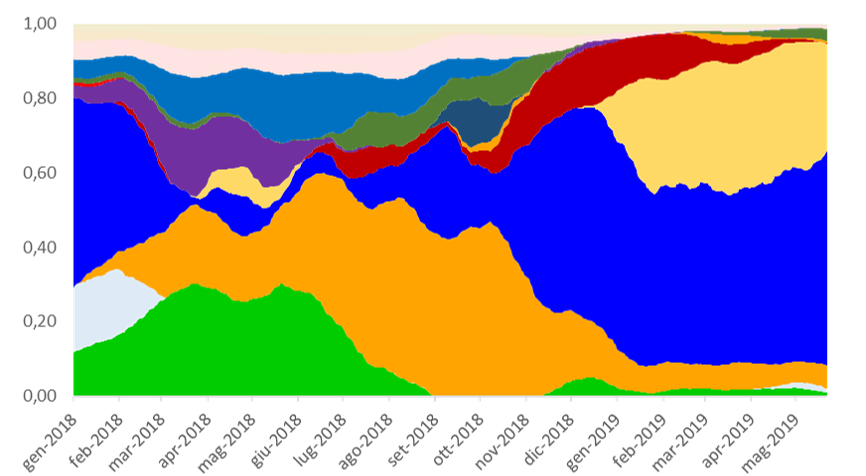
\includegraphics[width=3.2cm, height=2.6cm]{Images/rolling_allocation/rollstall.png}
            \end{figure}
		\end{column}
		\begin{column}{0.3\textwidth}  
		    \begin{center}
            \Fontvi{}\textcolor{blue}{Standard + btc}
            \end{center}
            \begin{figure}
                \centering
                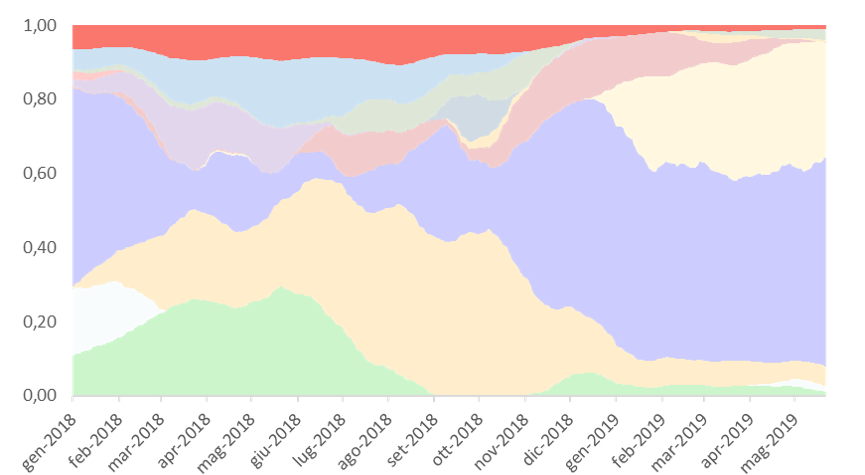
\includegraphics[width=3.2cm, height=2.6cm]{Images/rolling_allocation/rollcrbtc.png}
            \end{figure}
            \begin{figure}
                \centering
                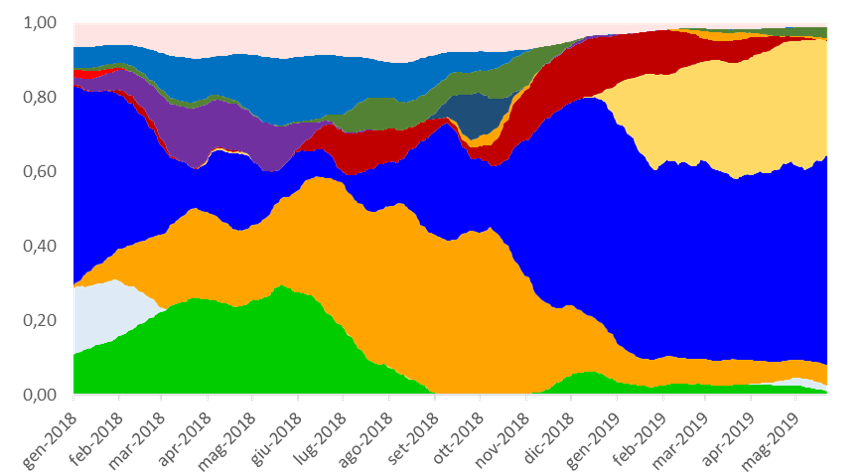
\includegraphics[width=3.2cm, height=2.6cm]{Images/rolling_allocation/rollstbtc.png}
            \end{figure}
		\end{column}
    	\begin{column}{0.3\textwidth} 
    	    \begin{center}
            \Fontvi{}Standard
            \end{center}
            \begin{figure}
                \centering
                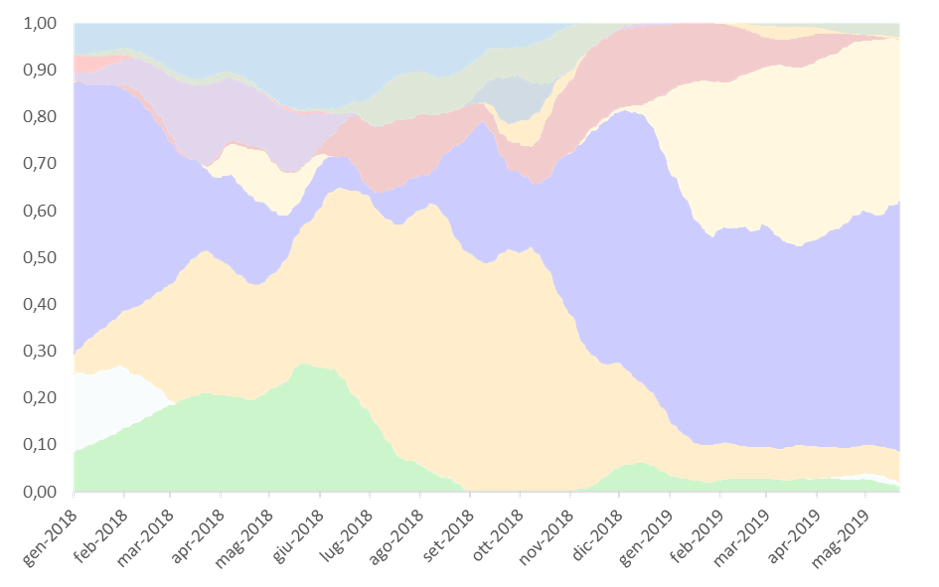
\includegraphics[width=3.2cm, height=2.6cm]{Images/rolling_allocation/rollcrno.png}
            \end{figure}
            \begin{figure}
                \centering
                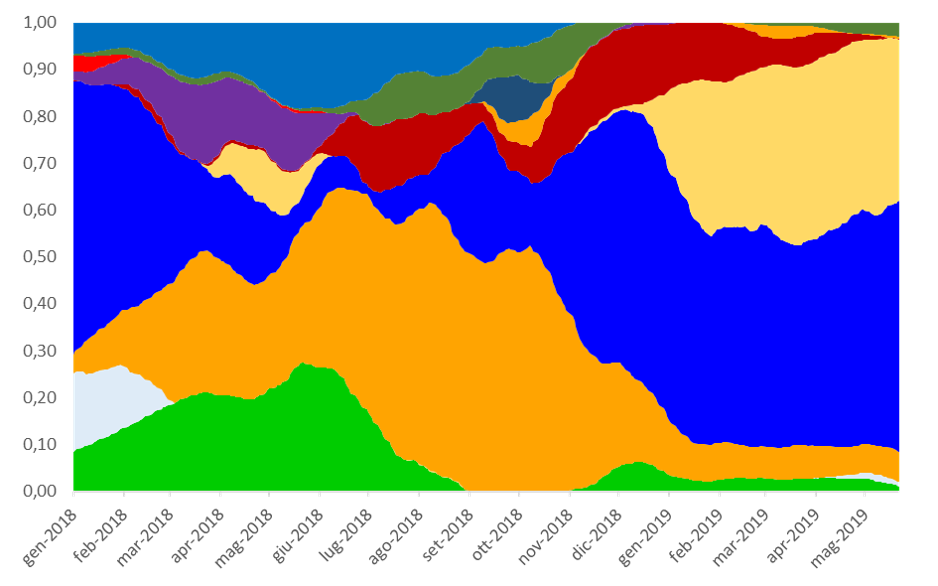
\includegraphics[width=3.2cm, height=2.6cm]{Images/rolling_allocation/rollstno.png}
            \end{figure}
		\end{column}
	\end{columns}
	\begin{figure}
	    \centering
	    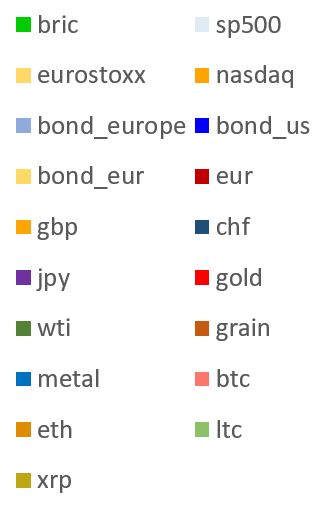
\includegraphics[width=\linewidth]{Images/legend.PNG}
	\end{figure}
\end{frame}



	
\section{Bibliography}

\begin{frame}[allowframebreaks] %allow to expand references to multiple frames (slides)
	\frametitle{References}

%	\scriptsize{\bibliographystyle{acm}}
%	
	\nocite{cr1}
	\nocite{trading}
	\nocite{correlations}
	\nocite{modernptftheory}
	\nocite{risk}
	\nocite{stazionario}
	\nocite{correl}
	\nocite{crosscorr}
	\nocite{spillover}
	\nocite{corr_stock}
	\nocite{weiyi}
	\nocite{BTC2008}
	\nocite{digitalgold}
	\nocite{klein}
	\nocite{bouri}
	\nocite{corbet}
	\nocite{mark52}
	\nocite{Fabozzi7}
	\nocite{DEoptimR_manual}
	\nocite{quadp}
	\nocite{R}
	\nocite{DEoptim_book}
	\nocite{Meucci}
	\nocite{mark59}
	\nocite{samuele}
	\nocite{CMC}
	\nocite{cryptoindex}
	\nocite{cryptoindex1}
	\bibliography{bibliography} %bibtex file name without .bib extension

\end{frame}

\section{Conclusions}


\begin{frame}{Conclusions}
	\begin{enumerate}
		\item Cryptoassets returns behave like standard assets returns: Fat tails and Volatility clustering 
		\bigskip
			
		\item Cryptoassets are a new asset class
		\bigskip
		
		\item In an optimal allocation framework cryptoassets generate value
		\bigskip
		
		\item To diversify among digital assets does not contribute to the value generation, thus it is convenient to bet on a single one of these assets
	\end{enumerate}	
\end{frame}


{
	\usebackgroundtemplate{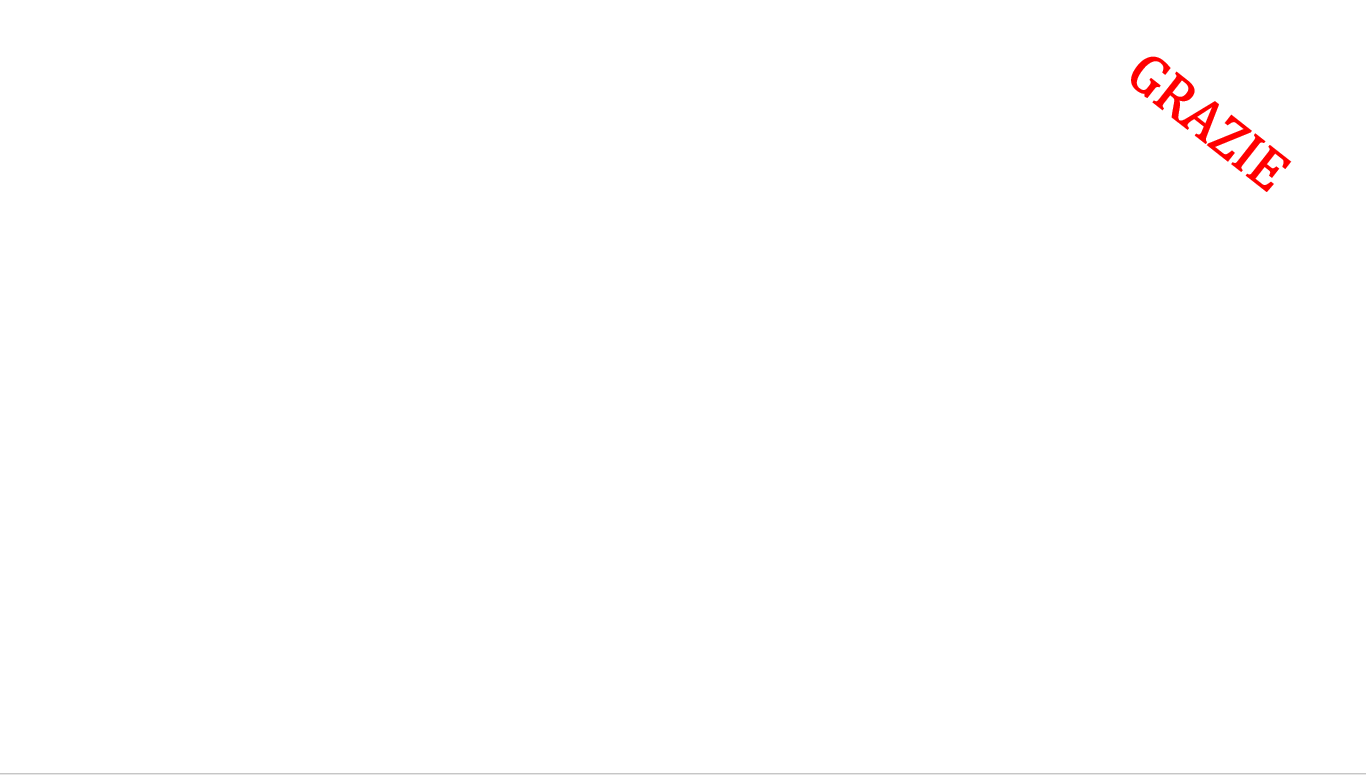
\includegraphics[width=\paperwidth,trim=4 4 4 4,clip]{Images/grazie.PNG}}%
	\begin{frame}{Conclusions}
	\begin{enumerate}
		\item Cryptoassets returns behave like standard assets returns: Fat tails and Volatility clustering 
		\bigskip
			
		\item Cryptoassets are a new asset class
		\bigskip
		
		\item In an optimal allocation framework cryptoassets generate value
		\bigskip
		
		\item To diversify among digital assets does not contribute to the value generation, thus it is convenient to bet on a single one of these assets
	\end{enumerate}	
    \end{frame}
}

\end{document}